\documentclass{article}
\usepackage[T1]{fontenc}
\usepackage{lmodern}
\usepackage{graphicx}
\usepackage{amsmath,amssymb}
\usepackage[a4paper,margin=2cm]{geometry}
\usepackage[absolute,overlay]{textpos}
\setlength{\TPHorizModule}{1mm}
\setlength{\TPVertModule}{1mm}
\usepackage[indonesian]{babel}
\usepackage{hyperref}
\setlength{\emergencystretch}{2em}
% unit: Halaman 109

\begin{document}

% === Halaman 109 (llm) ===

\vspace{95.04mm}

\section*{Enigma Rotors}

\vspace{10mm}

\begin{itemize}
    \item SPARE LIGHT BULBS
    \item VIEWING WINDOWS ON LID SHOW ENCODED LETTERS
    \item ROTOR CYLINDER CARRIES THREE AND LATER FOUR SCRAMBLER ROTORS
    \item POSITION OF ROTORS CONTROLS ENCODING OF EACH LETTER
    \item PLUGBOARD SETTINGS ARE CHANGED DAILY
    \item WOODEN CASE LID
    \item ALPHABETICAL LIGHTBOARD SHOWS FINAL ENCODED LETTERS
    \item KEYBOARD TO TYPE IN MESSAGE
\end{itemize}

% deskripsi: Foto mesin Enigma lengkap dengan label keterangan bagian-bagian utamanya seperti lampu, rotor, keyboard, dan plugboard.
% bbox normalisasi: [0.0200, 0.0000, 0.4300, 0.9800]
\begin{textblock*}{86.10mm}(4.20mm,0.00mm)
\noindent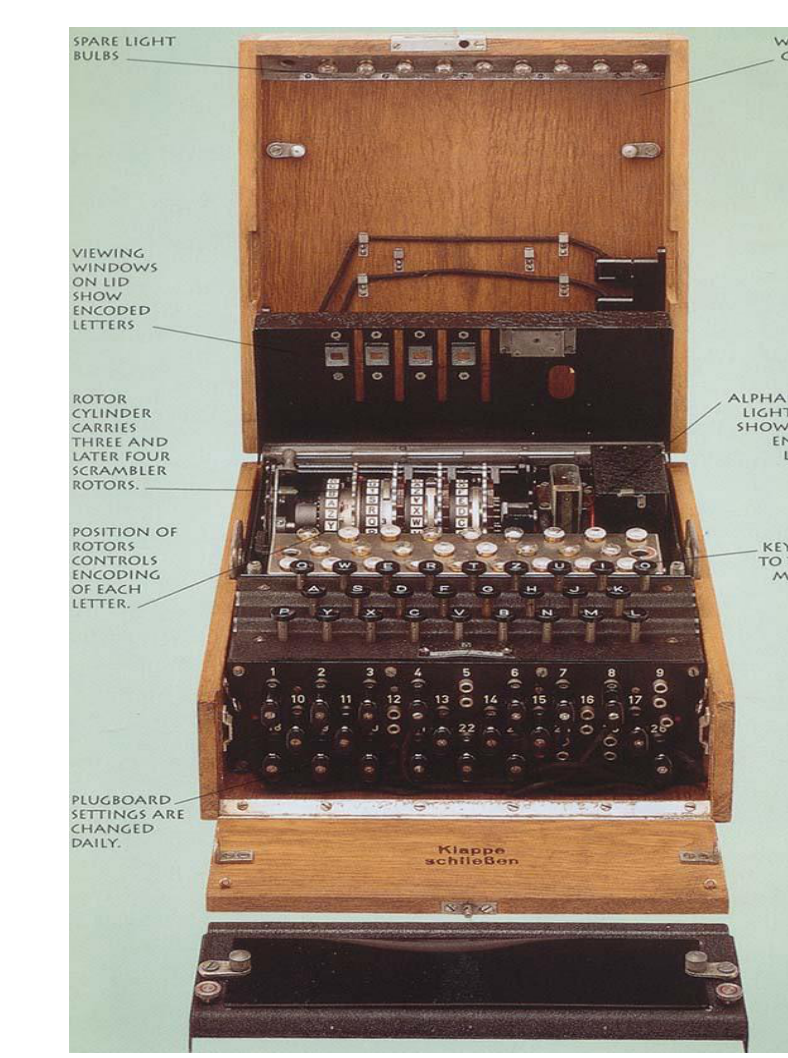
\includegraphics[width=86.10mm,height=291.06mm]{../../images/llm/page_109_img_01.png}%
\end{textblock*}

% deskripsi: Foto close-up bagian atas satu unit rotor Enigma yang menunjukkan kontak elektrik dan struktur gear.
% bbox normalisasi: [0.6000, 0.1100, 0.8300, 0.4300]
\begin{textblock*}{48.30mm}(126.00mm,32.67mm)
\noindent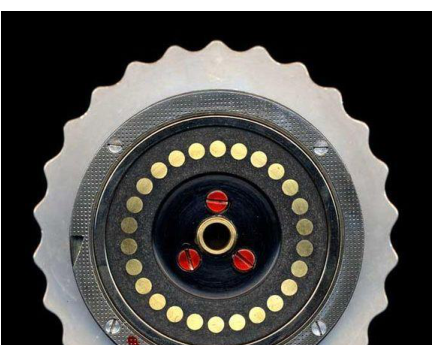
\includegraphics[width=48.30mm,height=95.04mm]{../../images/llm/page_109_img_02.png}%
\end{textblock*}

% deskripsi: Ilustrasi 3D dari rangkaian rotor Enigma yang menunjukkan susunan cakram alfabet dan poros penggeraknya.
% bbox normalisasi: [0.5900, 0.4600, 0.8500, 0.8500]
\begin{textblock*}{54.60mm}(123.90mm,136.62mm)
\noindent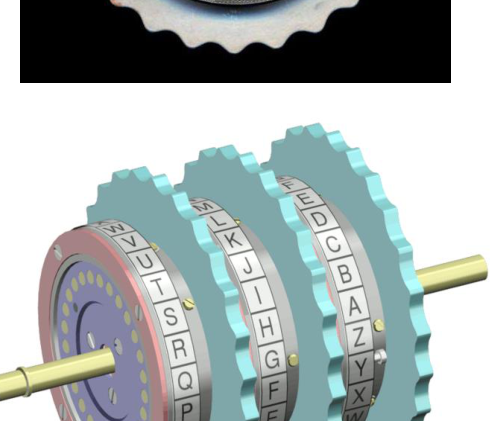
\includegraphics[width=54.60mm,height=115.83mm]{../../images/llm/page_109_img_03.png}%
\end{textblock*}

\end{document}
